\chapter{Geschäftsprozess ``Kaffeemaschine''}\label{ch:business-process}


\section{Beschreibung}\label{sec:beschreibung}
Unser Prozess soll die wichtigsten Abläufe rund um die Kaffeemaschine abdecken.
Dabei werden nur die Tasks abgebildet, die von der Maschine ausgeführt werden, nicht aber das jeweilige Verhalten des Benutzers.
Wir haben die folgenden Tasks bzw. Events für die Maschine definiert und umgesetzt:

\begin{longtable}{|p{.50\textwidth}|p{.50\textwidth}|}
    \hline
    \textbf{Task/Event} & \textbf{Beschreibung}
    \\ \hline
    Maschine einschalten & Die Maschine wird eingeschaltet und ist danach betriebsbereit.
    \\ \hline
    Maschine ausschalten & Die Maschine wird ausgeschaltet und kann danach (ausser einschalten) nicht mehr bedient werden.
    \\ \hline
    Zutaten auffüllen & Der Tank einer Zutat wird wieder gefüllt.
    Gilt für alle Zutaten.
    \\ \hline
    Bohnen mahlen & Die eingefüllten Bohnen werden gemahlen.
    Dies geschieht automatisch, nach dem Auffüllen der Bohnen.
    \\ \hline
    Kaffee herstellen & Die vom Benutzer gewählte Kaffeesorte wird hergestellt.
    Die Füllstände der für die Sorte benötigten Zutaten werden entsprechend reduziert.
    \\ \hline
    Füllstände überprüfen & Die Füllstände der Zutaten werden überprüft.
    Falls die Füllstände von gewissen Zutaten unter dem konfigurierten Limit sind, werden die betroffenen Zutaten auf dem Display angezeigt.
    \\ \hline
\end{longtable}\label{tab:tasks}


Die Kaffeemaschine bietet verschiedene Kaffeesorten an.
Alle Sorten werden aus einer Mischung der folgenden Zutaten hergestellt:
\begin{itemize}
    \item Wasser
    \item Bohnen
    \item Milch
    \item Zucker
\end{itemize}

In der folgenden Tabelle sind alle verfügbaren Kaffeesorten sowie die jeweiligen Mengen der Zutaten aufgeführt:

\begin{longtable}{|p{.20\textwidth}|p{.20\textwidth}|p{.20\textwidth}|p{.20\textwidth}|p{.20\textwidth}|}
    \hline
    \textbf{Sorte} & \textbf{Bohnen} & \textbf{Milch} & \textbf{Wasser} & \textbf{Zucker}
    \\ \hline
    Schwarz & 10 & 0 & 10 & 0
    \\ \hline
    Espresso & 5 & 0 & 5 & 0
    \\ \hline
    Mokka & 10 & 0 & 10 & 5
    \\ \hline
    Cappuccino & 10 & 10 & 5 & 0
    \\ \hline
    Latte Macciato & 15 & 10 & 15 & 0
    \\ \hline
    Milch (z.B. für Ovomaltine) & 0 & 20 & 0 & 0
    \\ \hline
\end{longtable}\label{tab:coffee-types}


\section{Diagramme}\label{sec:diagramme}
Wir haben den Prozess der Kaffeemaschine in zwei Diagrammen dargestellt.
Der grösste Teil des Prozesses ist im ``Coffe Simulator'' BPMN Diagramm abgebildet.
Die Entscheidung, wie viel von welcher Zutat für welche Kaffeesorte herausgelassen werden muss, haben wir in das ``Ingredients'' DMN Diagramm ausgelagert.
Folgend sind einige Ideen zu den genannten Diagrammen beschrieben.

\subsection{Coffee Simulator (BPMN)}\label{subsec:coffe-simulator-(bpmn)}
\begin{center}
    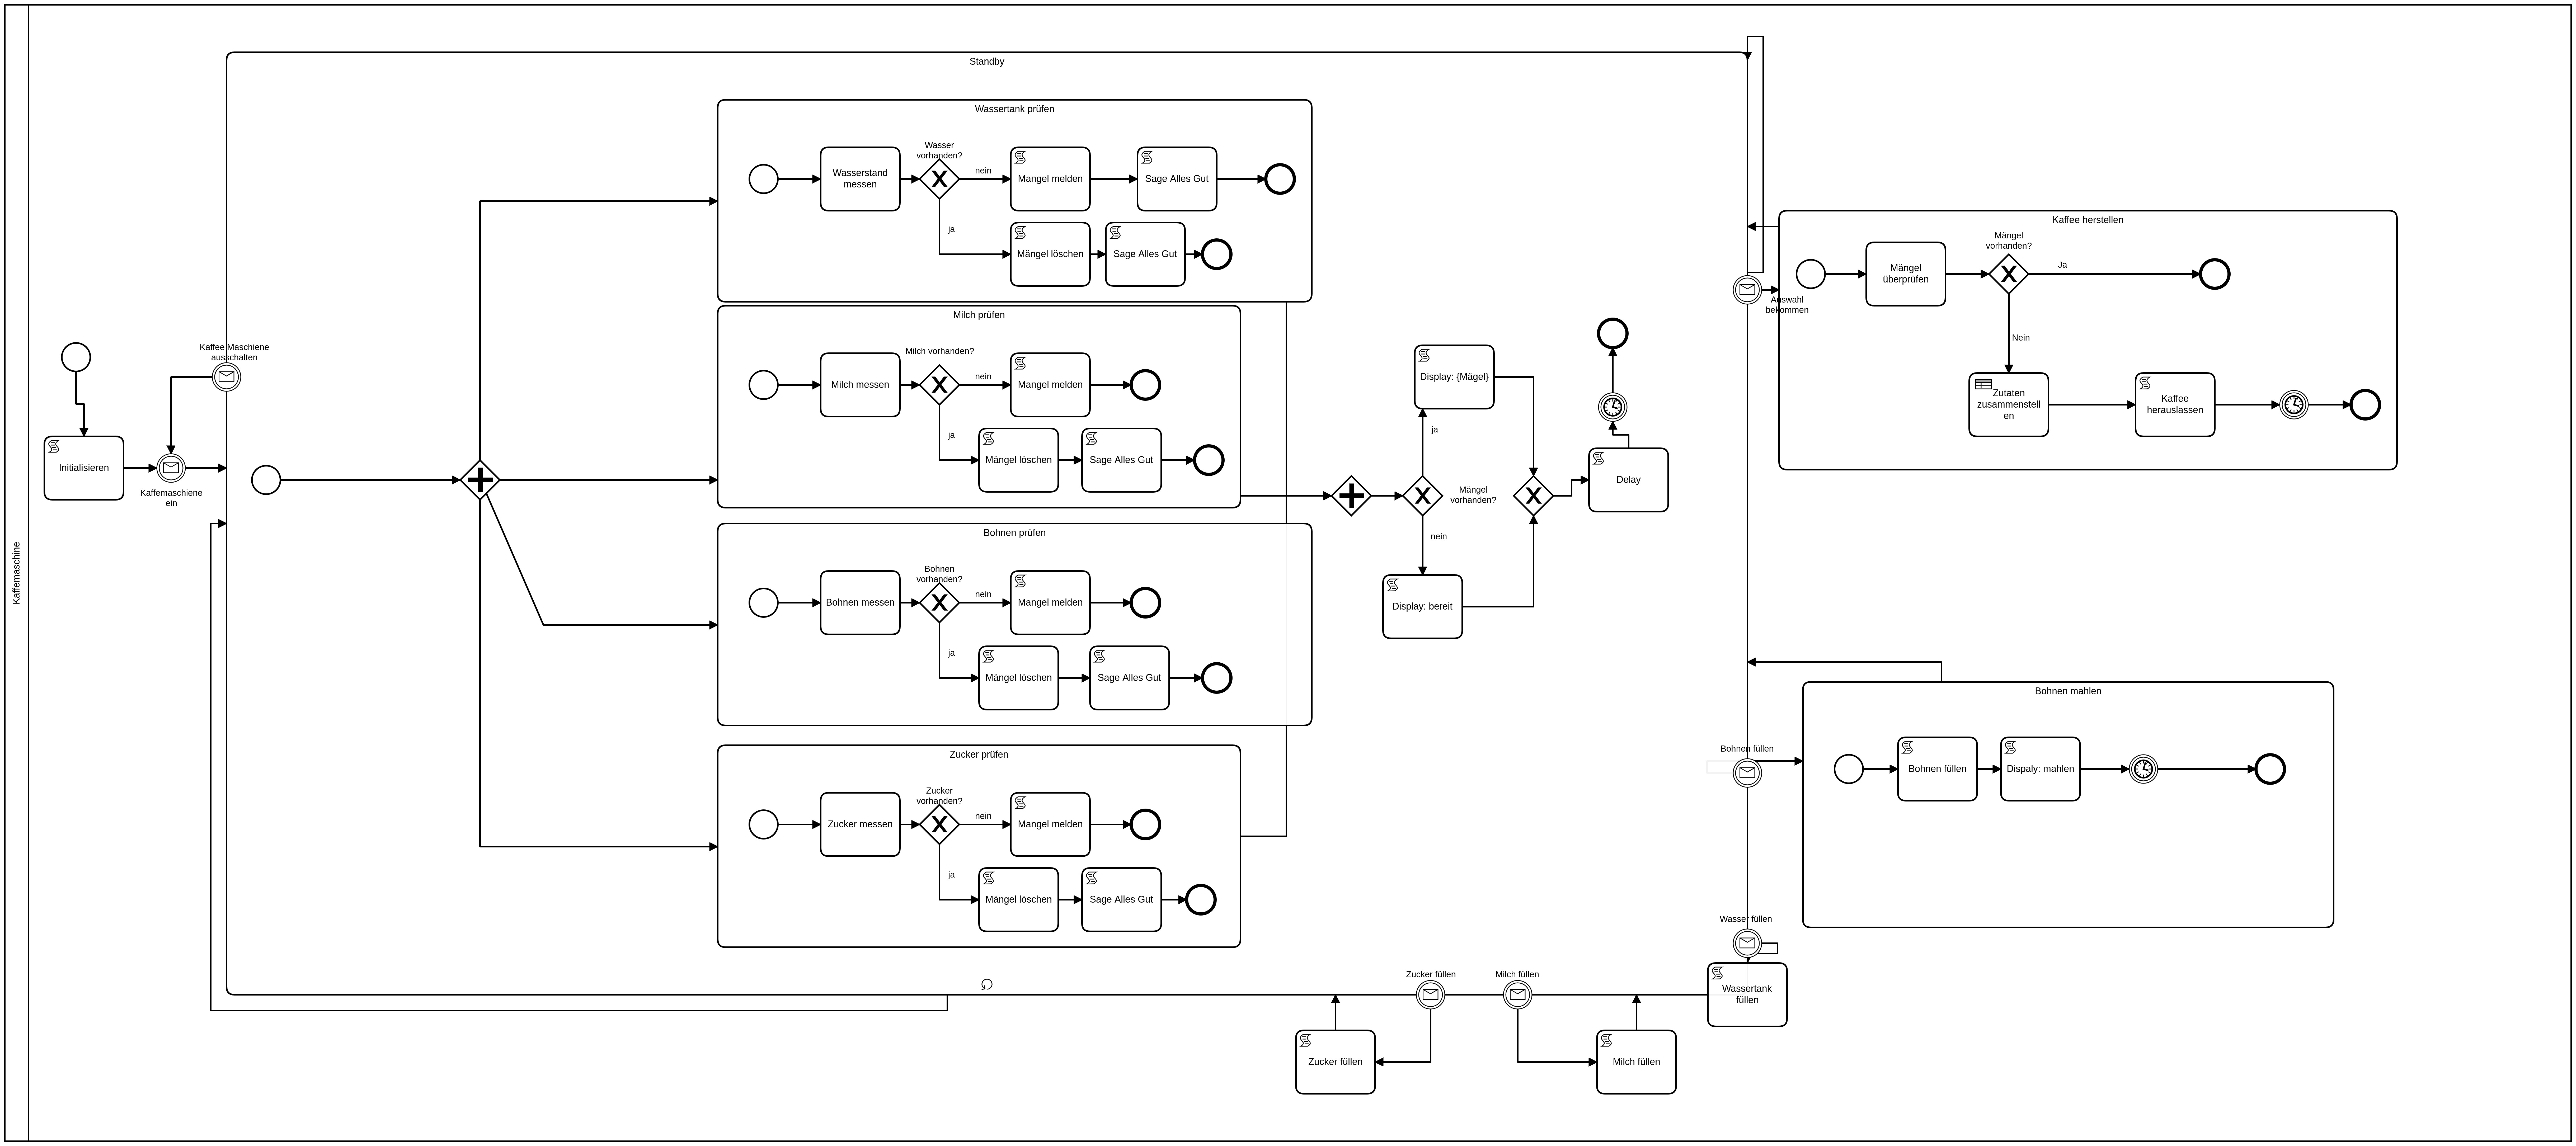
\includegraphics[width=1\textwidth]{resources/coffee_simulator_bpmn}
\end{center}

Dass Coffee Simulator BPMN Diagram enthält einen einzigen Prozess ``Kaffeemaschine''.
Beim Start des Prozesses werden die Prozessvariablen wie z.B. die Füllstände initialisiert, die Maschine ist aber noch ausgeschaltet.
Sobald die Maschine per Message eingeschaltet wird, wird der Sub-Prozess ``Standby'' gestartet, der sich unendlich oft wiederholt.
Im Standby-Zustand werden laufend die Füllstände überprüft und falls nötig als Mängel auf dem Display angezeigt.
Der Standby-Zustand kann durch verschiedene ``Boundry Message Events'' unterbrochen werden.
Beispiele von solchen Events sind das Herstellen eines Kaffees oder das Auffüllen eines Behälters.
In diesen Fällen wird der Standby-Prozess jeweils unterbrochen, der an den Event gekoppelte Task wird ausgeführt und schliesslich wird wieder in den Standby-Zustand gewechselt.
Eine Ausnahme bildet der Ausschalt-Event.
Dieser beendet den Standby-Zustand.

\subsection{Ingredients (DMN)}\label{subsec:ingredients-(dmn)}
\begin{center}
    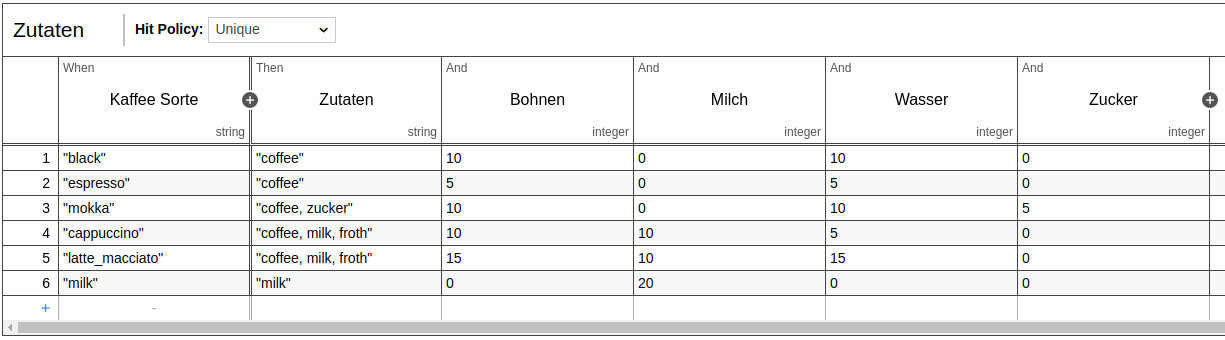
\includegraphics[width=1\textwidth]{resources/coffe_simulator_dmn}
\end{center}
Das Ingredients DMN wird verwendet, um die erforderlichen Zutaten für die verschiedenen Sorten zu ermitteln.
Es entspricht grundsätzlich der Tabelle~\ref{tab:coffee-types}.
Das DMN gibt die erforderliche Menge von jeder Zutat an den Prozess zurück, wo die Werte unteranderem verwendet werden, um die Füllstände anzupassen.

